% Short report for the base Ridge learning experiment.
% Numerical results are generated by scripts/ridge/analyze_sweep.jl.
\documentclass[11pt]{article}
\usepackage[margin=1in]{geometry}
\usepackage{booktabs}
\usepackage{graphicx}
\usepackage{microtype}
\usepackage{float}
\usepackage[T1]{fontenc}

% Generated by scripts/ridge/analyze_sweep.jl on 2026-09-07T12:41:56.998.
% Analysis commit: e3f041b8a284bda48bf98907d9f7b42521987b07
% Analysis source clean: true
% NN sweep: 2026-09-05_adeaa06_nn; commit: adeaa06f0b7098f8789925f0b638abddd935a16b
% Ridge sweep: 2026-09-06_c8f181f_ridge_pair_lambda_a0.001_lambda_b0.001; commit: c8f181fd7b5a8c6839a1e860fa34af9d56b72e12
% Effective realizations receive equal weight.
\newcommand{\rvDefine}[2]{\expandafter\newcommand\csname rv@#1\endcsname{#2}}
\newcommand{\rv}[1]{\csname rv@#1\endcsname}
\rvDefine{nConditions}{80}
\rvDefine{nCommonSeeds}{50}
\rvDefine{nOtherSeeds}{20}
\rvDefine{ridgeLambdaAgent}{0.001}
\rvDefine{ridgeLambdaBroker}{0.001}
\rvDefine{latePeriodStart}{481}
\rvDefine{latePeriodEnd}{500}
\rvDefine{mcLevelPercent}{95}
\rvDefine{summaryLowerPercent}{10}
\rvDefine{summaryUpperPercent}{90}
\rvDefine{rhoInteriorMin}{0.0}
\rvDefine{rhoInteriorMax}{0.85}
\rvDefine{rhoBoundary}{1.0}
\rvDefine{nnBaseline_agent_holdout_rank}{0.630}
\rvDefine{ridgeBaseline_agent_holdout_rank}{0.471}
\rvDefine{baselineDelta_agent_holdout_rank}{-0.160}
\rvDefine{baselineDeltaSE_agent_holdout_rank}{0.006}
\rvDefine{baselineDeltaLower_agent_holdout_rank}{-0.171}
\rvDefine{baselineDeltaUpper_agent_holdout_rank}{-0.148}
\rvDefine{nnBaseline_broker_holdout_rank}{0.948}
\rvDefine{ridgeBaseline_broker_holdout_rank}{0.845}
\rvDefine{baselineDelta_broker_holdout_rank}{-0.104}
\rvDefine{baselineDeltaSE_broker_holdout_rank}{0.005}
\rvDefine{baselineDeltaLower_broker_holdout_rank}{-0.114}
\rvDefine{baselineDeltaUpper_broker_holdout_rank}{-0.094}
\rvDefine{nnBaseline_rank_gap}{0.318}
\rvDefine{ridgeBaseline_rank_gap}{0.374}
\rvDefine{baselineDelta_rank_gap}{+0.056}
\rvDefine{baselineDeltaSE_rank_gap}{0.009}
\rvDefine{baselineDeltaLower_rank_gap}{+0.037}
\rvDefine{baselineDeltaUpper_rank_gap}{+0.074}
\rvDefine{nnBaseline_agent_holdout_r2}{-1.138}
\rvDefine{ridgeBaseline_agent_holdout_r2}{-2.627}
\rvDefine{baselineDelta_agent_holdout_r2}{-1.489}
\rvDefine{baselineDeltaSE_agent_holdout_r2}{0.054}
\rvDefine{baselineDeltaLower_agent_holdout_r2}{-1.598}
\rvDefine{baselineDeltaUpper_agent_holdout_r2}{-1.380}
\rvDefine{nnBaseline_broker_holdout_r2}{0.773}
\rvDefine{ridgeBaseline_broker_holdout_r2}{0.556}
\rvDefine{baselineDelta_broker_holdout_r2}{-0.217}
\rvDefine{baselineDeltaSE_broker_holdout_r2}{0.041}
\rvDefine{baselineDeltaLower_broker_holdout_r2}{-0.298}
\rvDefine{baselineDeltaUpper_broker_holdout_r2}{-0.135}
\rvDefine{nnBaseline_r2_gap}{1.911}
\rvDefine{ridgeBaseline_r2_gap}{3.183}
\rvDefine{baselineDelta_r2_gap}{+1.272}
\rvDefine{baselineDeltaSE_r2_gap}{0.071}
\rvDefine{baselineDeltaLower_r2_gap}{+1.129}
\rvDefine{baselineDeltaUpper_r2_gap}{+1.415}
\rvDefine{nnBaseline_output_gap}{1.713}
\rvDefine{ridgeBaseline_output_gap}{1.564}
\rvDefine{baselineDelta_output_gap}{-0.150}
\rvDefine{baselineDeltaSE_output_gap}{0.019}
\rvDefine{baselineDeltaLower_output_gap}{-0.188}
\rvDefine{baselineDeltaUpper_output_gap}{-0.111}
\rvDefine{nnBaseline_outsourcing_rate}{0.968}
\rvDefine{ridgeBaseline_outsourcing_rate}{0.942}
\rvDefine{baselineDelta_outsourcing_rate}{-0.026}
\rvDefine{baselineDeltaSE_outsourcing_rate}{0.004}
\rvDefine{baselineDeltaLower_outsourcing_rate}{-0.033}
\rvDefine{baselineDeltaUpper_outsourcing_rate}{-0.018}
\rvDefine{nnBaseline_access_fraction}{0.112}
\rvDefine{ridgeBaseline_access_fraction}{0.116}
\rvDefine{baselineDelta_access_fraction}{+0.005}
\rvDefine{baselineDeltaSE_access_fraction}{0.003}
\rvDefine{baselineDeltaLower_access_fraction}{-0.001}
\rvDefine{baselineDeltaUpper_access_fraction}{+0.010}
\rvDefine{nnBaseline_betweenness}{0.790}
\rvDefine{ridgeBaseline_betweenness}{0.749}
\rvDefine{baselineDelta_betweenness}{-0.041}
\rvDefine{baselineDeltaSE_betweenness}{0.006}
\rvDefine{baselineDeltaLower_betweenness}{-0.053}
\rvDefine{baselineDeltaUpper_betweenness}{-0.030}
\rvDefine{nnBaseline_mean_degree}{17.727}
\rvDefine{ridgeBaseline_mean_degree}{18.293}
\rvDefine{baselineDelta_mean_degree}{+0.567}
\rvDefine{baselineDeltaSE_mean_degree}{0.205}
\rvDefine{baselineDeltaLower_mean_degree}{+0.154}
\rvDefine{baselineDeltaUpper_mean_degree}{+0.980}
\rvDefine{nnMedian_agent_holdout_rank}{0.640}
\rvDefine{ridgeMedian_agent_holdout_rank}{0.476}
\rvDefine{deltaMean_agent_holdout_rank}{-0.146}
\rvDefine{deltaMedian_agent_holdout_rank}{-0.156}
\rvDefine{deltaQ10_agent_holdout_rank}{-0.238}
\rvDefine{deltaQ90_agent_holdout_rank}{-0.031}
\rvDefine{ridgeGreaterN_agent_holdout_rank}{0}
\rvDefine{nnPositiveN_agent_holdout_rank}{80}
\rvDefine{ridgePositiveN_agent_holdout_rank}{80}
\rvDefine{conditionCorrelation_agent_holdout_rank}{0.314}
\rvDefine{nnMedian_broker_holdout_rank}{0.940}
\rvDefine{ridgeMedian_broker_holdout_rank}{0.845}
\rvDefine{deltaMean_broker_holdout_rank}{-0.048}
\rvDefine{deltaMedian_broker_holdout_rank}{-0.042}
\rvDefine{deltaQ10_broker_holdout_rank}{-0.119}
\rvDefine{deltaQ90_broker_holdout_rank}{+0.033}
\rvDefine{ridgeGreaterN_broker_holdout_rank}{18}
\rvDefine{nnPositiveN_broker_holdout_rank}{80}
\rvDefine{ridgePositiveN_broker_holdout_rank}{80}
\rvDefine{conditionCorrelation_broker_holdout_rank}{0.671}
\rvDefine{nnMedian_rank_gap}{0.271}
\rvDefine{ridgeMedian_rank_gap}{0.354}
\rvDefine{deltaMean_rank_gap}{+0.099}
\rvDefine{deltaMedian_rank_gap}{+0.069}
\rvDefine{deltaQ10_rank_gap}{-0.038}
\rvDefine{deltaQ90_rank_gap}{+0.268}
\rvDefine{ridgeGreaterN_rank_gap}{64}
\rvDefine{nnPositiveN_rank_gap}{80}
\rvDefine{ridgePositiveN_rank_gap}{80}
\rvDefine{conditionCorrelation_rank_gap}{0.277}
\rvDefine{nnMedian_agent_holdout_r2}{-1.203}
\rvDefine{ridgeMedian_agent_holdout_r2}{-2.515}
\rvDefine{deltaMean_agent_holdout_r2}{-1.193}
\rvDefine{deltaMedian_agent_holdout_r2}{-1.503}
\rvDefine{deltaQ10_agent_holdout_r2}{-2.318}
\rvDefine{deltaQ90_agent_holdout_r2}{+0.883}
\rvDefine{ridgeGreaterN_agent_holdout_r2}{15}
\rvDefine{nnPositiveN_agent_holdout_r2}{0}
\rvDefine{ridgePositiveN_agent_holdout_r2}{0}
\rvDefine{conditionCorrelation_agent_holdout_r2}{-0.049}
\rvDefine{nnMedian_broker_holdout_r2}{0.589}
\rvDefine{ridgeMedian_broker_holdout_r2}{0.556}
\rvDefine{deltaMean_broker_holdout_r2}{+0.838}
\rvDefine{deltaMedian_broker_holdout_r2}{-0.035}
\rvDefine{deltaQ10_broker_holdout_r2}{-0.228}
\rvDefine{deltaQ90_broker_holdout_r2}{+3.340}
\rvDefine{ridgeGreaterN_broker_holdout_r2}{38}
\rvDefine{nnPositiveN_broker_holdout_r2}{58}
\rvDefine{ridgePositiveN_broker_holdout_r2}{75}
\rvDefine{conditionCorrelation_broker_holdout_r2}{0.520}
\rvDefine{nnMedian_r2_gap}{1.690}
\rvDefine{ridgeMedian_r2_gap}{3.124}
\rvDefine{deltaMean_r2_gap}{+2.032}
\rvDefine{deltaMedian_r2_gap}{+1.489}
\rvDefine{deltaQ10_r2_gap}{+0.205}
\rvDefine{deltaQ90_r2_gap}{+3.439}
\rvDefine{ridgeGreaterN_r2_gap}{74}
\rvDefine{nnPositiveN_r2_gap}{69}
\rvDefine{ridgePositiveN_r2_gap}{80}
\rvDefine{conditionCorrelation_r2_gap}{0.009}
\rvDefine{nnMedian_output_gap}{1.541}
\rvDefine{ridgeMedian_output_gap}{1.340}
\rvDefine{deltaMean_output_gap}{-0.220}
\rvDefine{deltaMedian_output_gap}{-0.201}
\rvDefine{deltaQ10_output_gap}{-0.415}
\rvDefine{deltaQ90_output_gap}{+0.047}
\rvDefine{ridgeGreaterN_output_gap}{11}
\rvDefine{nnPositiveN_output_gap}{66}
\rvDefine{ridgePositiveN_output_gap}{63}
\rvDefine{conditionCorrelation_output_gap}{0.979}
\rvDefine{nnMedian_outsourcing_rate}{0.963}
\rvDefine{ridgeMedian_outsourcing_rate}{0.934}
\rvDefine{deltaMean_outsourcing_rate}{-0.010}
\rvDefine{deltaMedian_outsourcing_rate}{-0.018}
\rvDefine{deltaQ10_outsourcing_rate}{-0.047}
\rvDefine{deltaQ90_outsourcing_rate}{+0.031}
\rvDefine{ridgeGreaterN_outsourcing_rate}{25}
\rvDefine{nnPositiveN_outsourcing_rate}{80}
\rvDefine{ridgePositiveN_outsourcing_rate}{80}
\rvDefine{conditionCorrelation_outsourcing_rate}{0.984}
\rvDefine{nnMedian_access_fraction}{0.105}
\rvDefine{ridgeMedian_access_fraction}{0.115}
\rvDefine{deltaMean_access_fraction}{+0.007}
\rvDefine{deltaMedian_access_fraction}{+0.004}
\rvDefine{deltaQ10_access_fraction}{-0.002}
\rvDefine{deltaQ90_access_fraction}{+0.021}
\rvDefine{ridgeGreaterN_access_fraction}{63}
\rvDefine{nnPositiveN_access_fraction}{80}
\rvDefine{ridgePositiveN_access_fraction}{80}
\rvDefine{conditionCorrelation_access_fraction}{0.981}
\rvDefine{nnMedian_betweenness}{0.765}
\rvDefine{ridgeMedian_betweenness}{0.724}
\rvDefine{deltaMean_betweenness}{-0.027}
\rvDefine{deltaMedian_betweenness}{-0.033}
\rvDefine{deltaQ10_betweenness}{-0.059}
\rvDefine{deltaQ90_betweenness}{+0.008}
\rvDefine{ridgeGreaterN_betweenness}{14}
\rvDefine{nnPositiveN_betweenness}{80}
\rvDefine{ridgePositiveN_betweenness}{80}
\rvDefine{conditionCorrelation_betweenness}{0.997}
\rvDefine{nnMedian_mean_degree}{17.710}
\rvDefine{ridgeMedian_mean_degree}{19.093}
\rvDefine{deltaMean_mean_degree}{+1.899}
\rvDefine{deltaMedian_mean_degree}{+1.027}
\rvDefine{deltaQ10_mean_degree}{-0.473}
\rvDefine{deltaQ90_mean_degree}{+3.502}
\rvDefine{ridgeGreaterN_mean_degree}{68}
\rvDefine{nnPositiveN_mean_degree}{80}
\rvDefine{ridgePositiveN_mean_degree}{80}
\rvDefine{conditionCorrelation_mean_degree}{0.990}

% Generated by scripts/ridge/paired_figures.jl on 2026-09-14T13:14:46.340.
% Rendering commit: 79fd29611cc083f703ba36f36b371c473695cf20
\newcommand{\rfvDefine}[2]{\expandafter\newcommand\csname rfv@#1\endcsname{#2}}
\newcommand{\rfv}[1]{\csname rfv@#1\endcsname}
\rfvDefine{rollingWindow}{5}
\rfvDefine{networkMeasureInterval}{20}
\rfvDefine{displayStart}{30}


\title{Base Ridge Learning Experiment}
\author{}
\date{}

\begin{document}
\maketitle
\renewcommand{\thefigure}{R\arabic{figure}}
\renewcommand{\thetable}{R\arabic{table}}

\paragraph{Question and design.}
This experiment asks whether the broker's ranking advantage persists when both
agents and the broker use Ridge regression instead of neural networks. Agents
predict match quality from the candidate's type. The broker uses additive and
bilinear features of the pair and pools its mediated-match history. Thus, the
experiment tests whether neural-network flexibility is necessary for a broker
ranking advantage while retaining each learner's information and feature map.
The calibrated penalties are $\lambda_a=\rv{ridgeLambdaAgent}$ and
$\lambda_b=\rv{ridgeLambdaBroker}$.

The primary estimand in realization $c$ is
\[
G_L(c)=\overline{r}_{b,L}(c)-\overline{r}_{a,L}(c),
\]
where $L\in\{\mathrm{NN},\mathrm{Ridge}\}$ and each bar is the seed-averaged
holdout rank correlation over periods \rv{latePeriodStart}--\rv{latePeriodEnd}.
The learning-system contrast is
$G_{\mathrm{Ridge}}(c)-G_{\mathrm{NN}}(c)$. It includes the endogenous changes
in matching and later learning histories induced by the learning rule. It is
not a fixed-data comparison of estimators. Each of the
\rv{nConditions} effective realizations receives one observation. Grid
coordinates that refer to the same realization receive no additional weight.
The model comparison uses the same seeds in both learning conditions:
\rv{nCommonSeeds} at the baseline and \rv{nOtherSeeds} elsewhere.

Figures~\ref{fig:ridge-dynamics}--\ref{fig:ridge-advantage} reproduce the
corresponding main figures with NN and base Ridge on shared axes.
Figure~\ref{fig:ridge-comparison} shows paired comparisons of the primary
ranking and output outcomes.

\paragraph{Baseline.}
With the common seeds, the NN broker-minus-principal difference in holdout rank
correlation is \rv{nnBaseline_rank_gap}, compared with
\rv{ridgeBaseline_rank_gap} under base Ridge. The paired change is
\rv{baselineDelta_rank_gap}, with a \rv{mcLevelPercent}\% Monte Carlo interval of
[\rv{baselineDeltaLower_rank_gap}, \rv{baselineDeltaUpper_rank_gap}].
Table~\ref{tab:ridge-baseline} reports other baseline outcomes.
Figure~\ref{fig:ridge-dynamics} shows the full baseline dynamics, and
Figure~\ref{fig:ridge-comparison}A isolates the broker and agent ranking trajectories.

\begin{table}[ht]
\centering
\caption{Baseline late-period outcomes under NN and base Ridge learning}
\label{tab:ridge-baseline}
\begin{tabular}{lrrr}
\toprule
Outcome & NN & Ridge & Ridge $-$ NN \\
\midrule
Agent holdout rank correlation
  & \rv{nnBaseline_agent_holdout_rank}
  & \rv{ridgeBaseline_agent_holdout_rank}
  & \rv{baselineDelta_agent_holdout_rank} \\
Broker holdout rank correlation
  & \rv{nnBaseline_broker_holdout_rank}
  & \rv{ridgeBaseline_broker_holdout_rank}
  & \rv{baselineDelta_broker_holdout_rank} \\
Broker-minus-principal difference in holdout rank correlation
  & \rv{nnBaseline_rank_gap}
  & \rv{ridgeBaseline_rank_gap}
  & \rv{baselineDelta_rank_gap} \\
Brokered-minus-self output gap
  & \rv{nnBaseline_output_gap}
  & \rv{ridgeBaseline_output_gap}
  & \rv{baselineDelta_output_gap} \\
Outsourcing rate
  & \rv{nnBaseline_outsourcing_rate}
  & \rv{ridgeBaseline_outsourcing_rate}
  & \rv{baselineDelta_outsourcing_rate} \\
Broker access fraction
  & \rv{nnBaseline_access_fraction}
  & \rv{ridgeBaseline_access_fraction}
  & \rv{baselineDelta_access_fraction} \\
Broker betweenness centrality
  & \rv{nnBaseline_betweenness}
  & \rv{ridgeBaseline_betweenness}
  & \rv{baselineDelta_betweenness} \\
\bottomrule
\end{tabular}
\begin{minipage}{0.92\linewidth}
\footnotesize
Entries use the \rv{nCommonSeeds} common seeds. Each seed is first averaged over
periods \rv{latePeriodStart}--\rv{latePeriodEnd}. The Ridge-minus-NN column is
the mean paired seed difference.
The access fraction is the share of accepted broker offers whose counterparty
was not already the demander's neighbor.
\end{minipage}
\end{table}

\paragraph{Robustness across model realizations.}
Across the \rv{nConditions} effective realizations, the median
broker-minus-principal difference in holdout rank correlation is
\rv{nnMedian_rank_gap} for NN and
\rv{ridgeMedian_rank_gap} for Ridge. The median Ridge-minus-NN contrast is
\rv{deltaMedian_rank_gap}. Its \rv{summaryLowerPercent}th and
\rv{summaryUpperPercent}th percentiles are
\rv{deltaQ10_rank_gap} and \rv{deltaQ90_rank_gap}. The Ridge difference is positive in
\rv{ridgePositiveN_rank_gap} realizations, compared with
\rv{nnPositiveN_rank_gap} under NN, and exceeds the NN difference in
\rv{ridgeGreaterN_rank_gap} realizations. The correlation between NN and Ridge
condition-level differences in holdout rank correlation is
\rv{conditionCorrelation_rank_gap}.

The within-system brokered-minus-self output gap has medians of
\rv{nnMedian_output_gap} under NN and \rv{ridgeMedian_output_gap} under Ridge.
Its median Ridge-minus-NN contrast is \rv{deltaMedian_output_gap}, and Ridge
exceeds NN in \rv{ridgeGreaterN_output_gap} realizations. This channel mean
difference is descriptive, not a causal estimate of the value of brokerage:
channel choice, candidate sets, and offer acceptance are endogenous. Median
outsourcing is \rv{nnMedian_outsourcing_rate} under NN and
\rv{ridgeMedian_outsourcing_rate} under Ridge.

Figure~\ref{fig:ridge-grid} shows the matching-problem surface under each
learning system. Figure~\ref{fig:ridge-position} compares the broker's network
position and access. Figure~\ref{fig:ridge-advantage} relates the ranking and
output differences to those structural outcomes. Figure~\ref{fig:ridge-comparison}B--C
shows the paired condition-level changes directly against zero.

\paragraph{Interpretation.}
Neural-network flexibility is not necessary for the broker to rank candidates
better than agents in this modeled system. The Ridge broker-minus-principal
difference is positive in \rv{ridgePositiveN_rank_gap} of \rv{nConditions}
effective realizations. This experiment does not identify the source of that
advantage because the broker still observes both parties, represents pairs with
additive and bilinear features, and pools mediated-match observations. The
ablation experiment restricts these features separately.

\clearpage
\section*{Illustrative figures}

\begin{figure}[H]
\centering
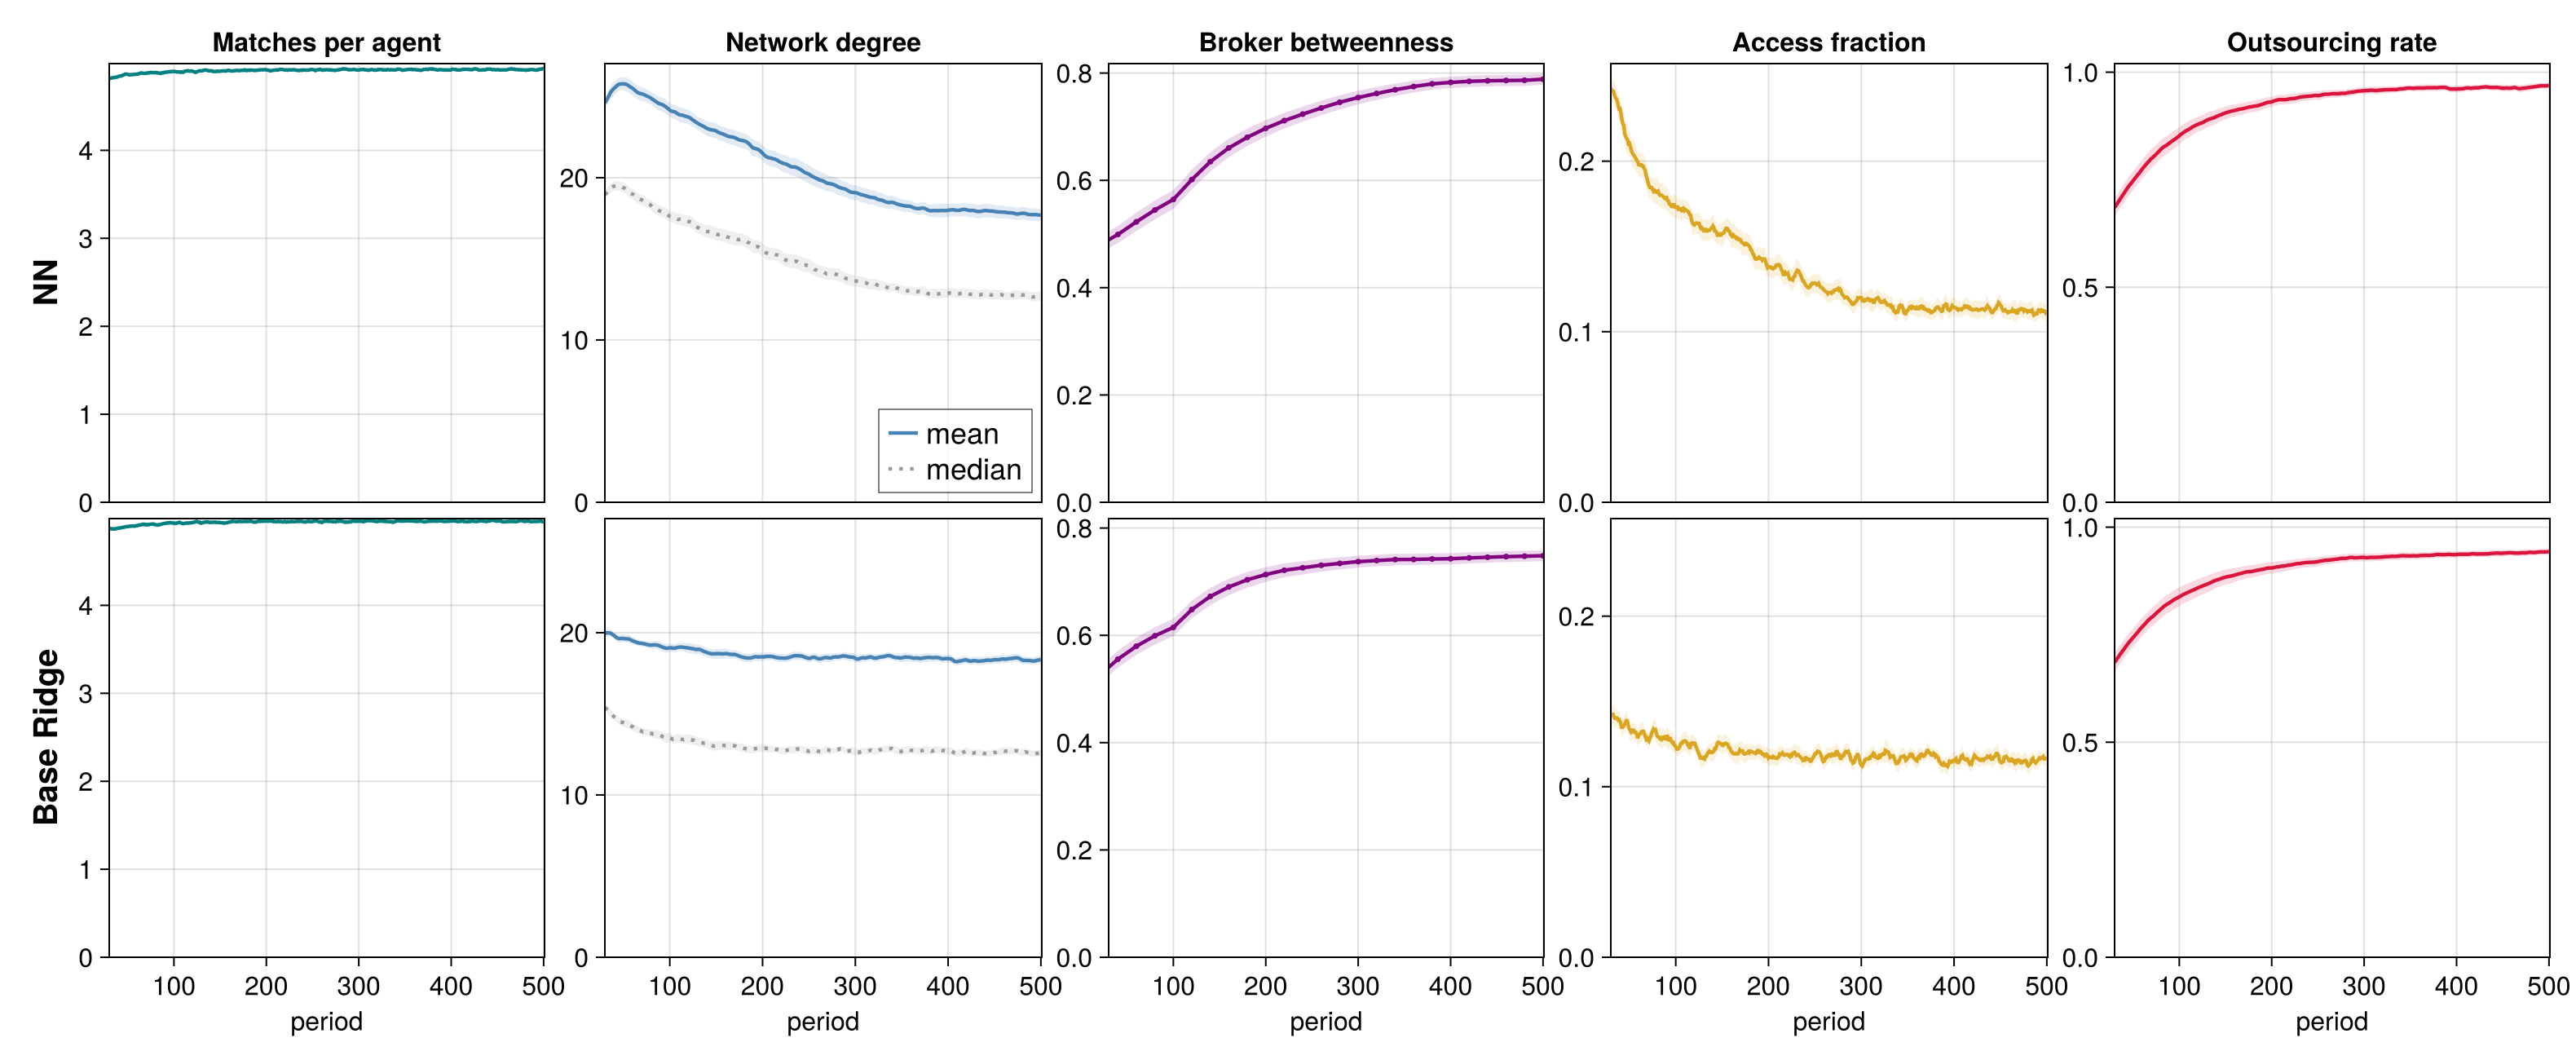
\includegraphics[width=\linewidth]{../output/ridge/paired/figures/baseline_dynamics.png}
\caption{Baseline dynamics under NN and base Ridge. Rows identify the
learning system. Panels show matches per agent, mean and median agent-network
degree, broker betweenness centrality, access fraction, and outsourcing rate.
Lines are \rfv{rollingWindow}-observation rolling ensemble means over
\rv{nCommonSeeds} common seeds. Ribbons are pointwise
\rv{mcLevelPercent}\% Monte Carlo intervals. Betweenness is measured every
\rfv{networkMeasureInterval} periods; other measures are recorded every period.
Axes begin at period \rfv{displayStart} and are shared across learning systems.}
\label{fig:ridge-dynamics}
\end{figure}

\begin{figure}[H]
\centering
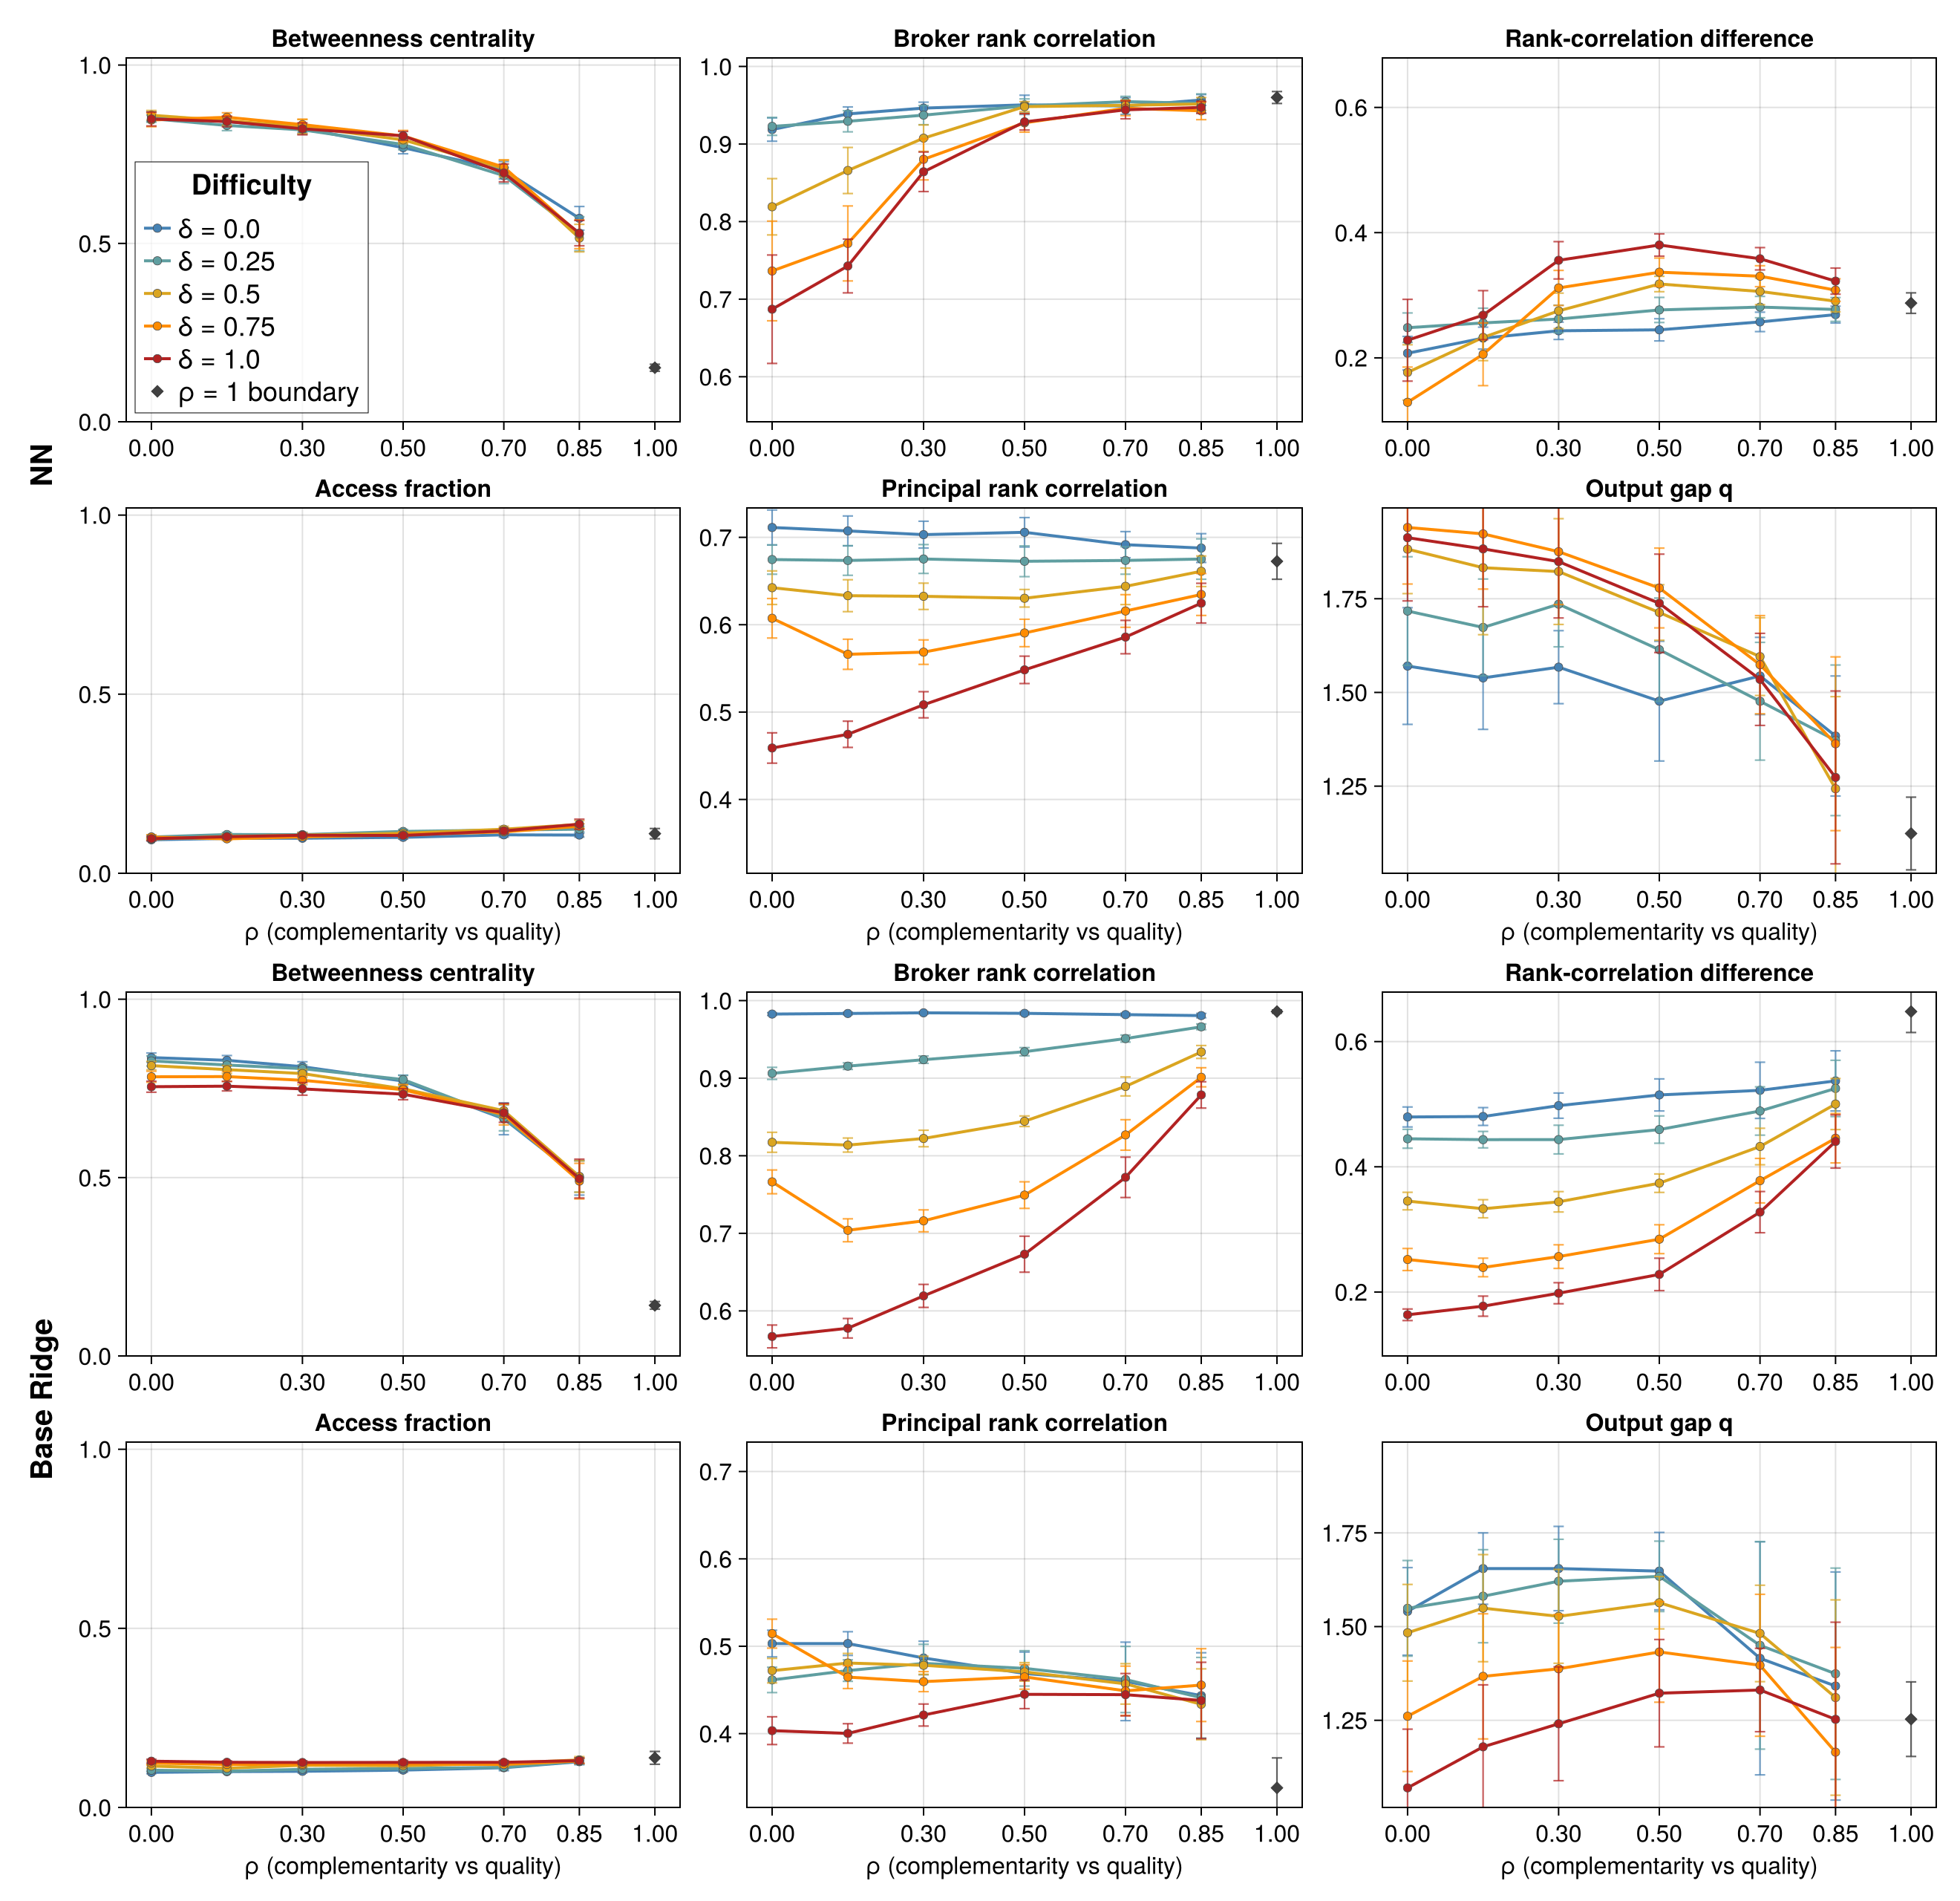
\includegraphics[width=\linewidth]{../output/ridge/paired/figures/matching_grid.png}
\caption{Outcomes across the $\rho\times\delta$ matching grid under NN (top
two rows) and base Ridge (bottom two rows). Each line is a value of $\delta$;
lines span $\rho=\rv{rhoInteriorMin}$ through $\rv{rhoInteriorMax}$. The
pure-quality boundary $\rho=\rv{rhoBoundary}$, where
$\delta$ is inactive, is shown once and unconnected. Each marker is an effective
realization's late-window seed mean. Corresponding NN and Ridge panels use the
same vertical scale. Whiskers are \rv{mcLevelPercent}\% Monte Carlo intervals.}
\label{fig:ridge-grid}
\end{figure}

\begin{figure}[H]
\centering
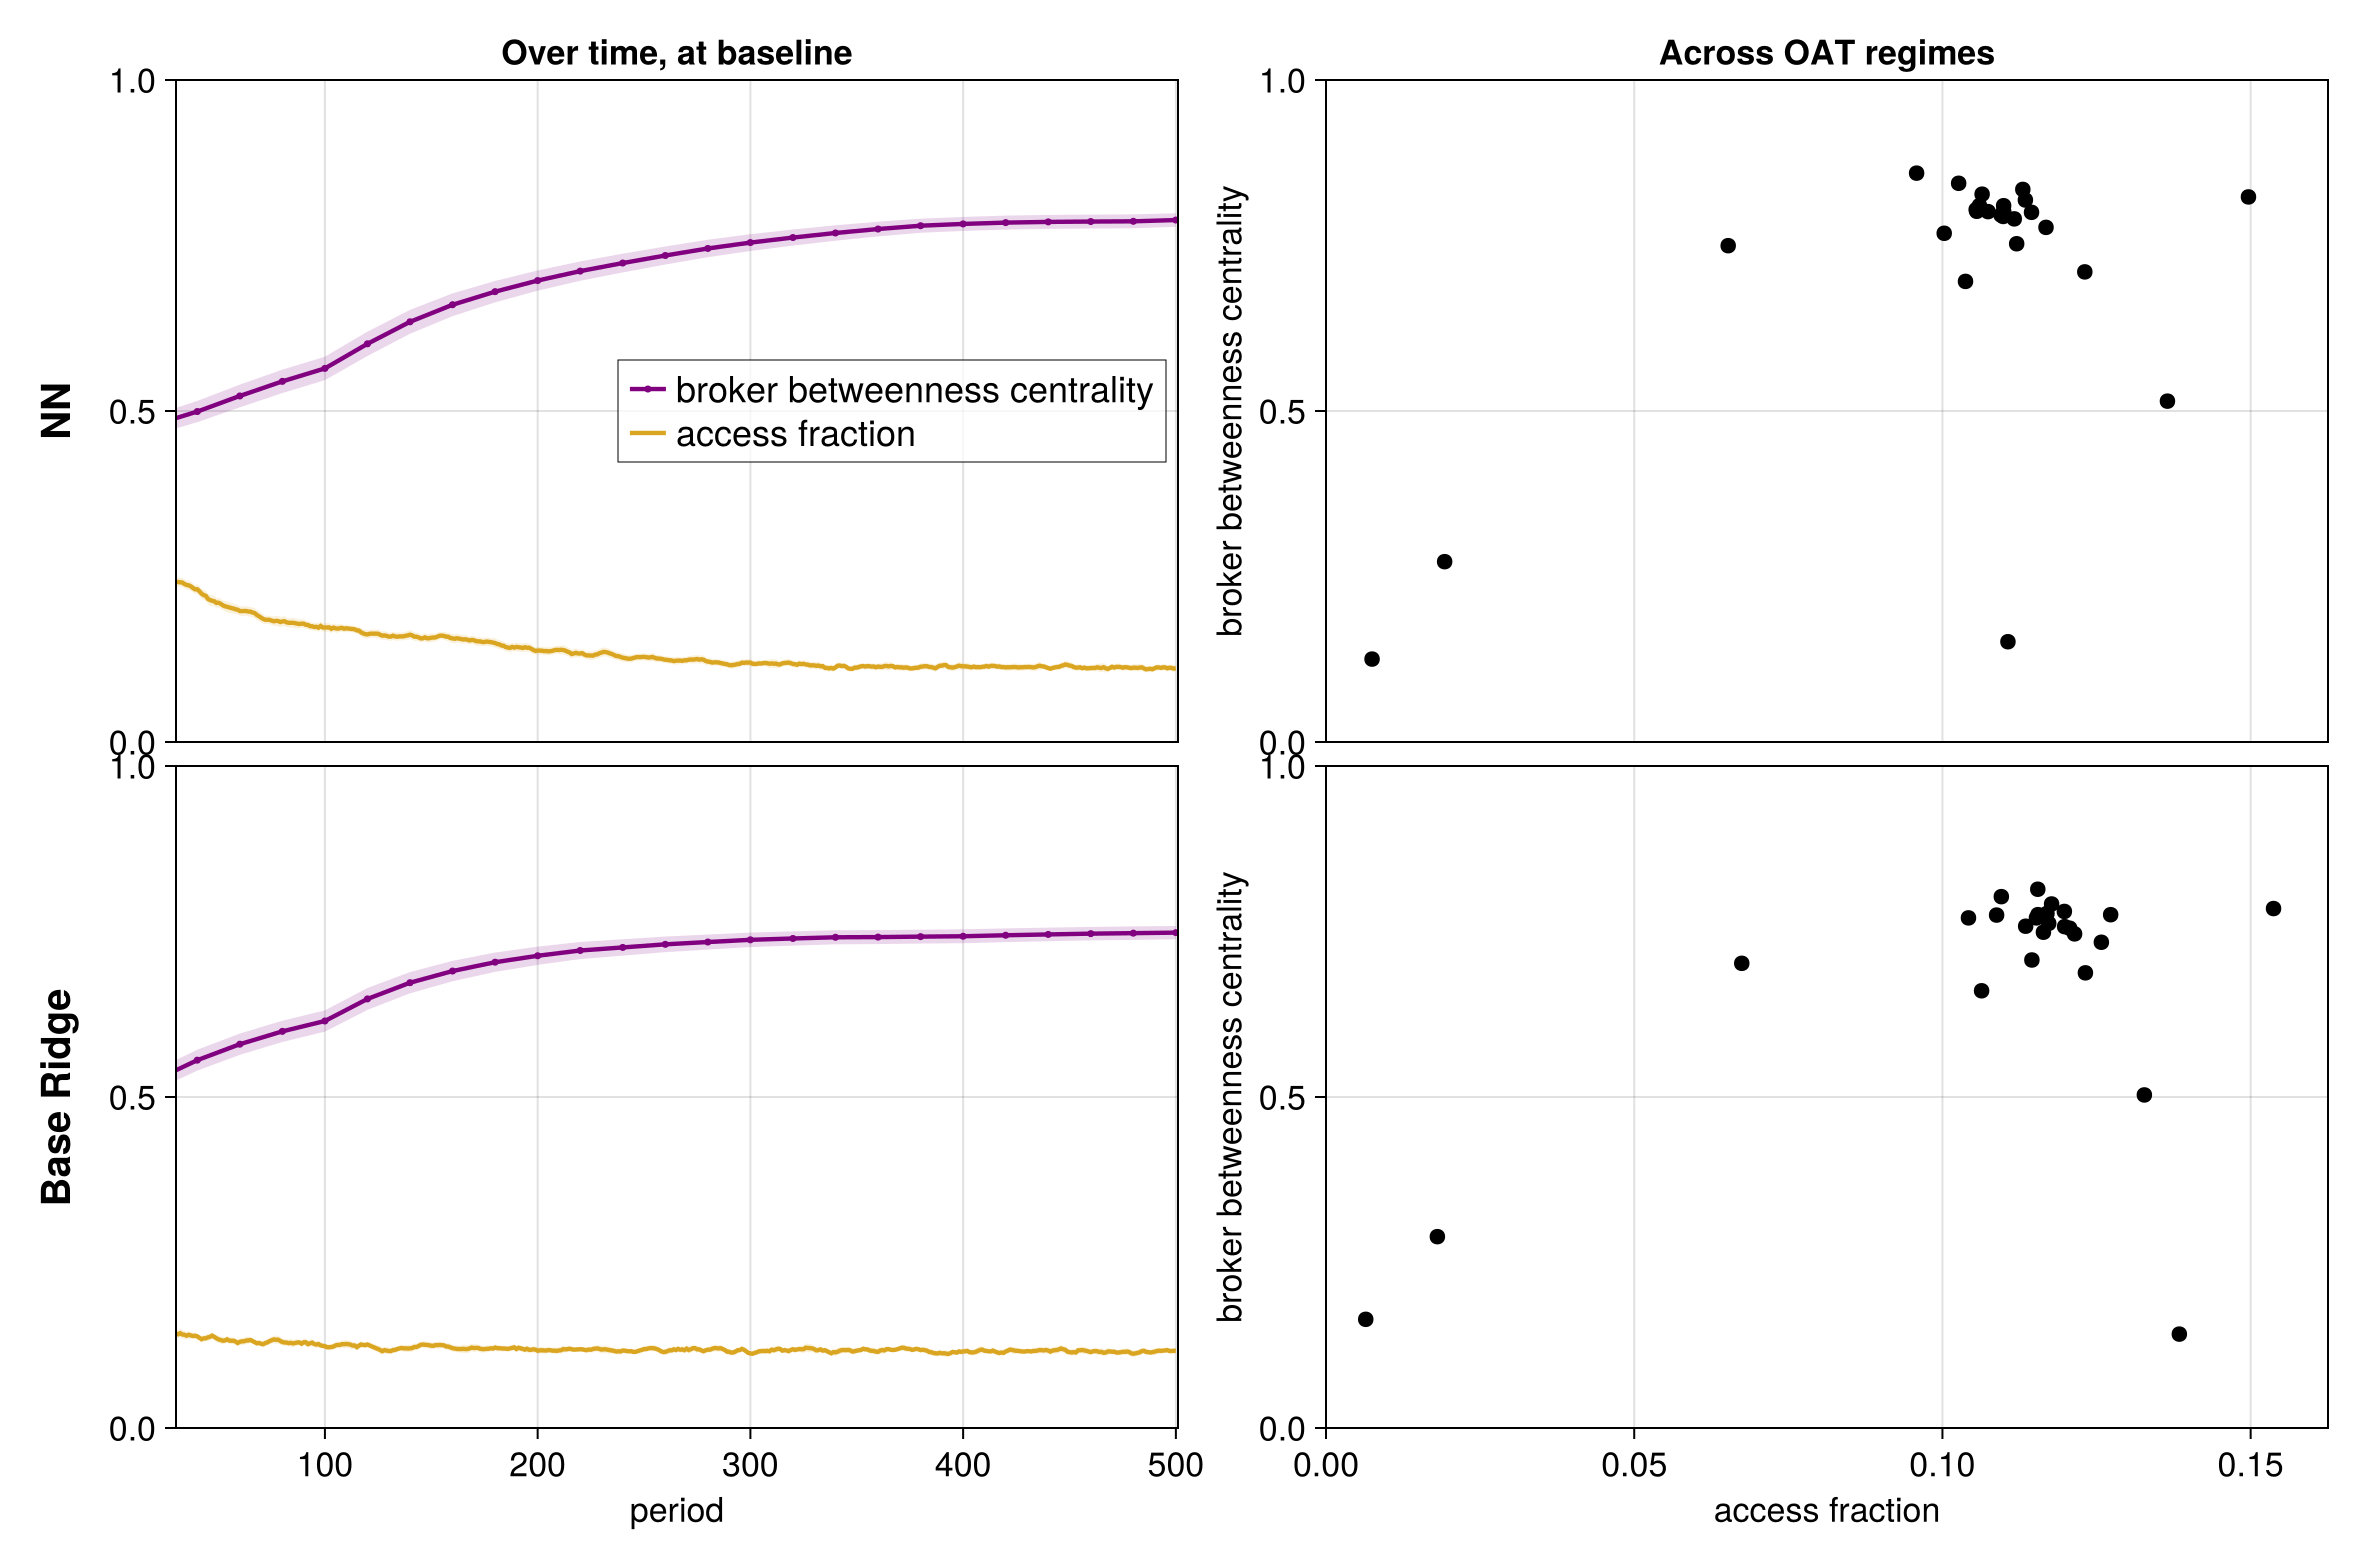
\includegraphics[width=\linewidth]{../output/ridge/paired/figures/centrality_and_access.png}
\caption{Broker position and access under NN and base Ridge. Left panels show
\rfv{rollingWindow}-observation rolling ensemble means at the baseline. Right panels show one
point per one-at-a-time regime, using late-window seed means. Ribbons are
pointwise \rv{mcLevelPercent}\% Monte Carlo intervals. Corresponding
panels use shared axes.}
\label{fig:ridge-position}
\end{figure}

\clearpage
\begin{figure}[H]
\centering
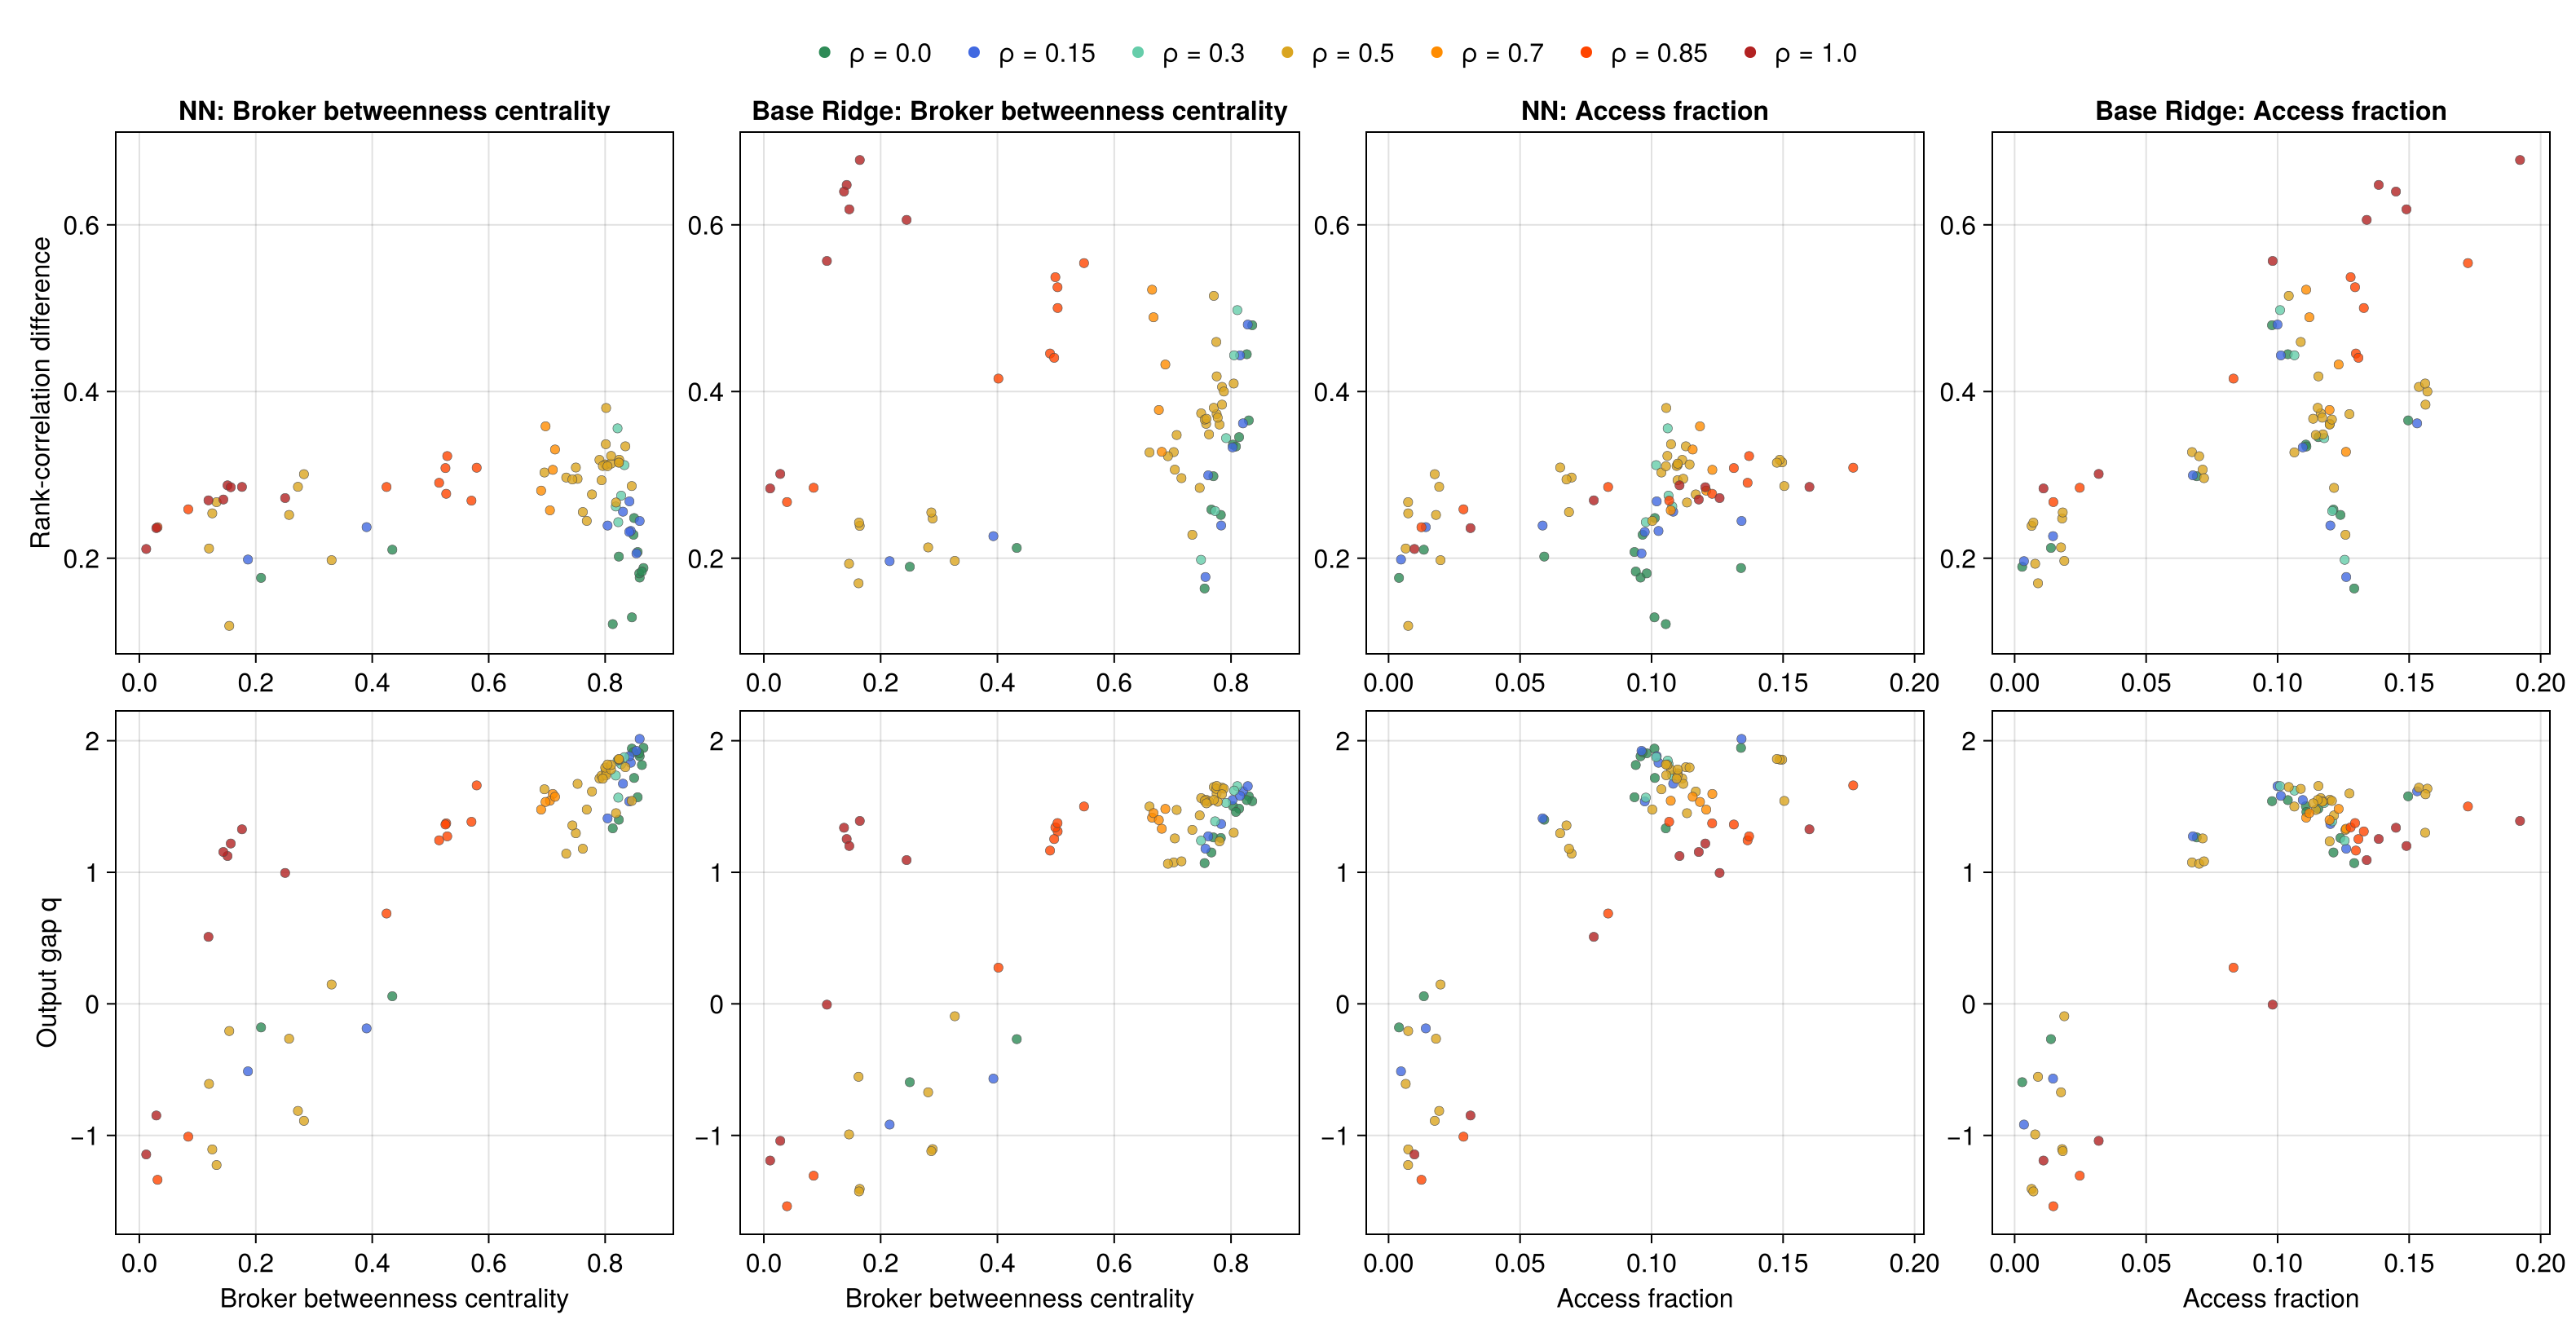
\includegraphics[width=\linewidth]{../output/ridge/paired/figures/structural_advantage.png}
\caption{Broker-minus-principal differences in holdout rank correlation and
brokered-minus-self output gaps against broker
betweenness centrality and access fraction under NN and base Ridge. Each
point is one effective realization's late-window seed mean. Corresponding NN
and Ridge panels use shared axes; color denotes $\rho$.}
\label{fig:ridge-advantage}
\end{figure}

\begin{figure}[H]
\centering
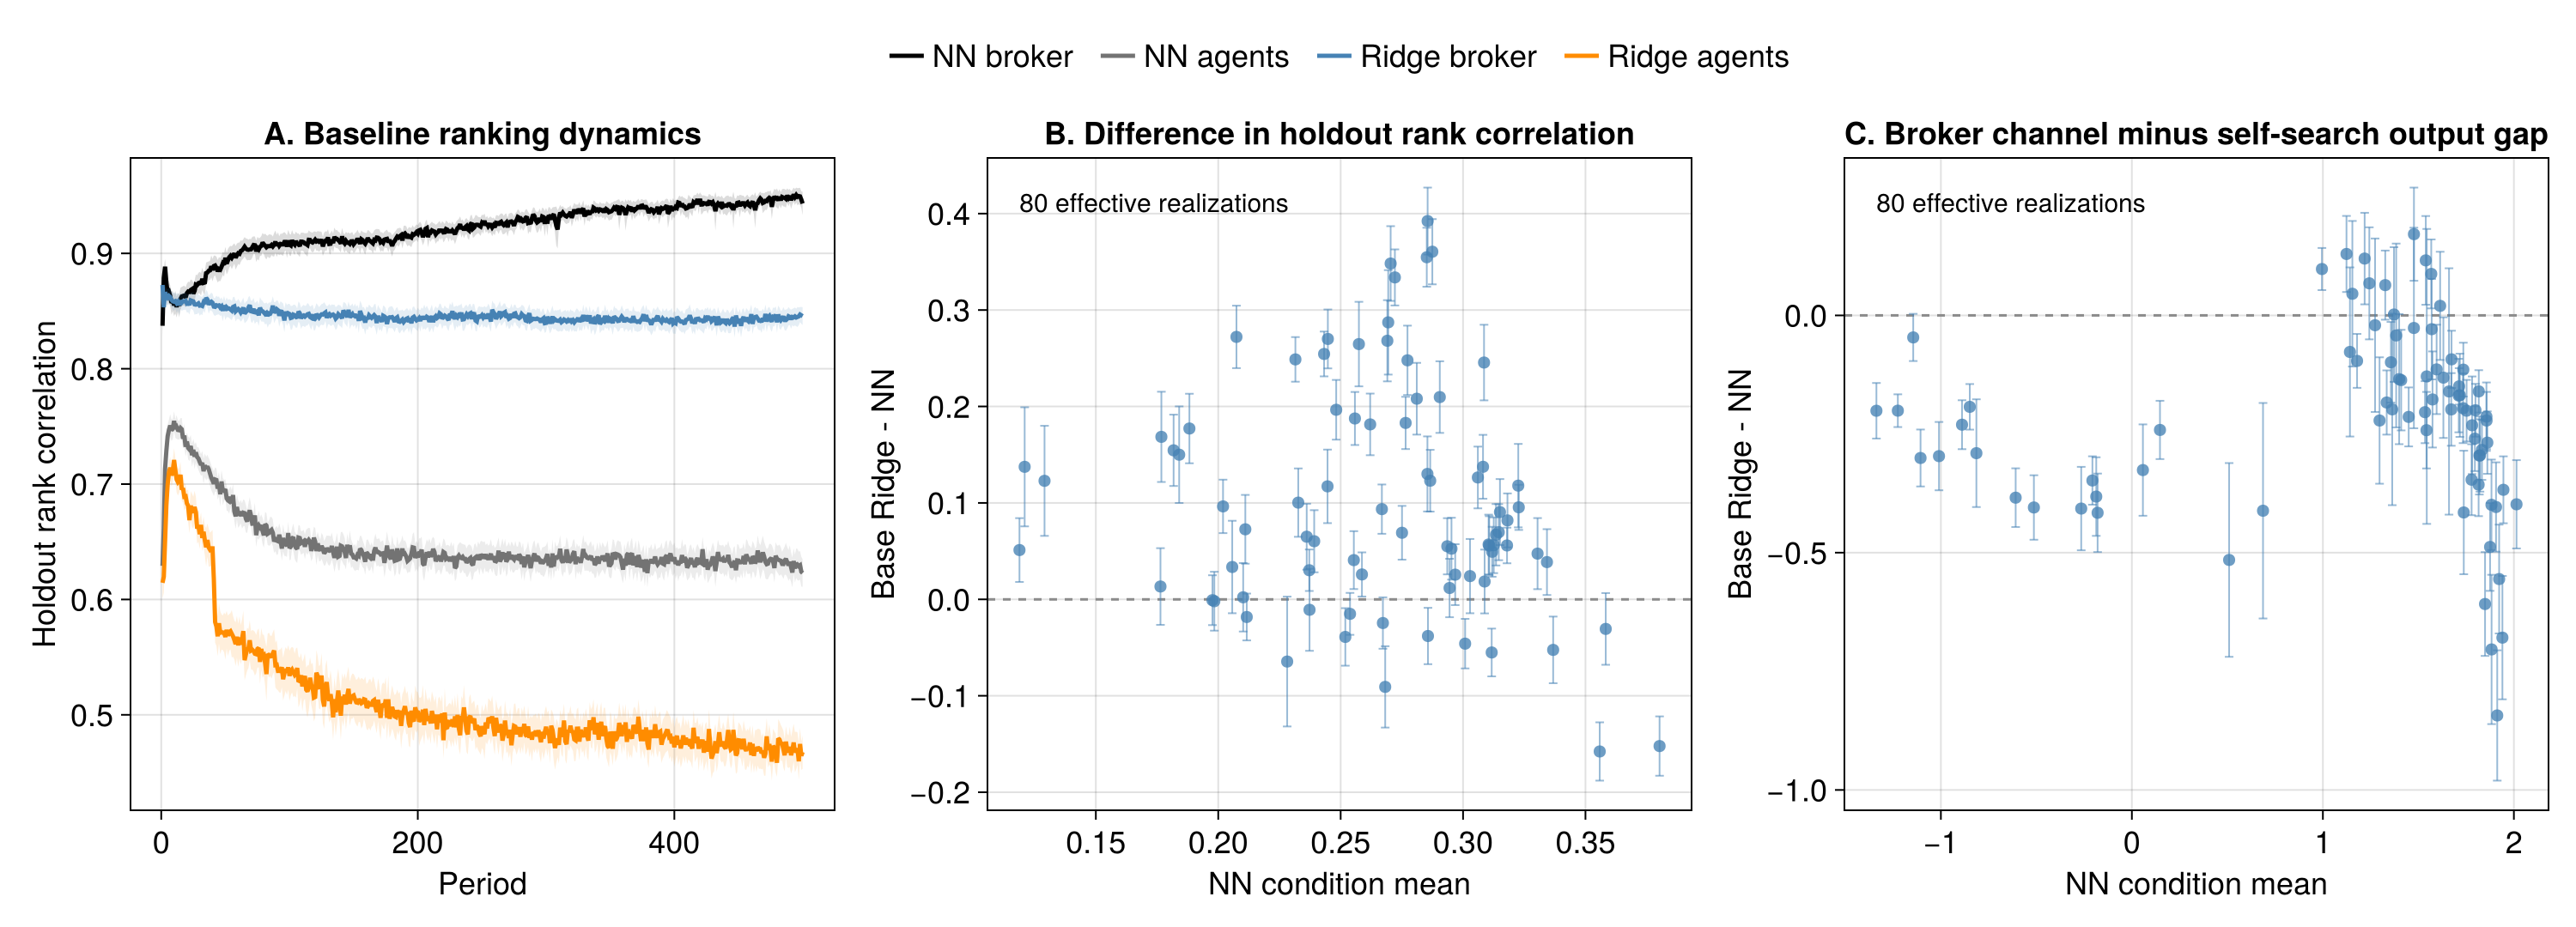
\includegraphics[width=\linewidth]{../output/ridge/paired/figures/ridge_comparison.png}
\caption{Direct comparison of NN and base Ridge. Panel A shows broker and principal
holdout rank correlation over time under NN and base Ridge at the baseline.
Lines are ensemble means over \rv{nCommonSeeds} common seeds; ribbons are pointwise
\rv{mcLevelPercent}\% Monte
Carlo intervals. Panels B and C show the paired change from NN to base Ridge in the
broker-minus-principal difference in holdout rank correlation and in the broker
channel-minus-self-search output gap, respectively, for each of the
\rv{nConditions} effective
realizations. The horizontal position is that realization's NN mean. Whiskers are
paired \rv{mcLevelPercent}\% Monte Carlo intervals for the mean seed-level change, and dashed lines
mark no change.}
\label{fig:ridge-comparison}
\end{figure}

\end{document}
